%; whizzy paragraph -pdf xpdf -latex ./whizzypdfptex.sh
%; whizzy-paragraph "^\\\\begin{frame}"
% latex beamer presentation.
% platex, latex-beamer でコンパイルすることを想定。 

%     Tokyo Debian Meeting resources
%     Copyright (C) 2009 Junichi Uekawa
%     Copyright (C) 2009 Nobuhiro Iwamatsu

%     This program is free software; you can redistribute it and/or modify
%     it under the terms of the GNU General Public License as published by
%     the Free Software Foundation; either version 2 of the License, or
%     (at your option) any later version.

%     This program is distributed in the hope that it will be useful,
%     but WITHOUT ANY WARRANTY; without even the implied warranty of
%     MERCHANTABILITY or FITNESS FOR A PARTICULAR PURPOSE.  See the
%     GNU General Public License for more details.

%     You should have received a copy of the GNU General Public License
%     along with this program; if not, write to the Free Software
%     Foundation, Inc., 51 Franklin St, Fifth Floor, Boston, MA  02110-1301 USA

\documentclass[cjk,dvipdfmx,12pt]{beamer}
\usetheme{Tokyo}
\usepackage{monthlypresentation}
%  preview (shell-command (concat "evince " (replace-regexp-in-string "tex$" "pdf"(buffer-file-name)) "&"))
%  presentation (shell-command (concat "xpdf -fullscreen " (replace-regexp-in-string "tex$" "pdf"(buffer-file-name)) "&"))
%  presentation (shell-command (concat "evince " (replace-regexp-in-string "tex$" "pdf"(buffer-file-name)) "&"))

%http://www.naney.org/diki/dk/hyperref.html
%日本語EUC系環境の時
\AtBeginDvi{\special{pdf:tounicode EUC-UCS2}}
%シフトJIS系環境の時
%\AtBeginDvi{\special{pdf:tounicode 90ms-RKSJ-UCS2}}

\title{東京エリア Debian 勉強会}
\subtitle{資料}
\author{岩松 信洋 iwamatsu@debian.or.jp\\IRC nick: iwamatsu}
\date{2009年11月14日}
\logo{
\includegraphics[width=8cm]{image200607/openlogo-light.eps}}

\begin{document}

\frame{\titlepage{}}

\emtext{設営準備にご協力ください}

\section{}
\begin{frame}
 \frametitle{Agenda}
\begin{minipage}[t]{0.45\hsize}
  \begin{itemize}
  \item 注意事項
	\begin{itemize}
	 \item 飲食禁止
	\end{itemize}
  \item 最近あったDebian関連のイベント報告
	\begin{itemize}
	 \item 前回の勉強会
	\end{itemize}
 \end{itemize}
\end{minipage} 
\begin{minipage}[t]{0.45\hsize}
 \begin{itemize}
  \item Debian Quiz
  \item Debian ではじめる数学事始め
  \item Debian autobuilder
 \end{itemize}
\end{minipage}
\end{frame}


\begin{frame}
 \frametitle{2009年10月}
\begin{minipage}[t]{0.45\hsize}
  \begin{itemize}
  \item 注意事項
	\begin{itemize}
	 \item 飲食禁止
	\end{itemize}
  \item 最近あったDebian関連のイベント報告
	\begin{itemize}
	 \item 前回の勉強会
	\end{itemize}
 \end{itemize}
\end{minipage} 
\begin{minipage}[t]{0.45\hsize}
 \begin{itemize}
  \item OSC2009 Tokyo / fall
  \item KOF 2009
 \end{itemize}
\end{minipage}
\end{frame}

\begin{frame}{Hack Cafe}

毎週水曜日、週に一回東京のどっかのカフェでハック。\\
\url{http://twitter.com/debian_hackcafe}\\
関西でも始めたようです。
\end{frame}

\begin{frame}{2009年計画}

{\scriptsize
 \begin{enumerate}
  \item 新年の企画 (アンサンブル荻窪開催)
  \item OSC Tokyo
  \item VAIO P インストール記録、
	カーネル読書会 ディストリビューション大集合(小林さん)(東京大学?)
  \item Git Handson (岩松)(あんさんぶる荻窪?)
  \item 家Debianサーバ vs 職場のネットワーク(千代田区都立図書館?\footnote{\url{http://www.library.chiyoda.tokyo.jp/}})
  \item DDTSS 
  \item スペインにて開催
  \item Debconf報告会
  \item Asterisk (東京大学?)、udev + HAL
  \item OSC Fall? (10月30・31日)
  \item 3D graphics 開発 
  \item Debian サーバ+VMware + 各種OS、
	他の仮想化ツール(vserver etc.)、
	忘年会
 \end{enumerate}
}
\end{frame}

\emtext{事前課題}

\begin{frame}{事前課題}
\begin{enumerate}
 \item あなたが普段行っている統計処理の内容とその処理で行っているハックを披露してください
\end{enumerate}
\end{frame}

{\footnotesize
%; whizzy-master ../debianmeetingresume200911.tex
% $B0J>e$N@_Dj$r$7$F$$$k$?$a!"$3$N%U%!%$%k$G(B M-x whizzytex $B$9$k$H!"(Bwhizzytex$B$,MxMQ$G$-$^$9!#(B

\begin{prework}{hoge}
\preworksection{hoge}


\end{prework}

\begin{prework}{fuga}

\preworksection{fuga}

\end{prework}

\begin{prework}{$B$^$($@$3$&$X$$(B}
\preworksection{$B$^$($@$3$&$X$$(B}

 $B8=>l$K$$$k$H$-$O$"$^$jI,MW$H$7$J$+$C$?$N$G$9$,!":rG/EY$^$G$N%W%j%;!<%k%9(B
 $B$N$H$-$O!"%W%m%S%8%g%K%s%0$9$k>e$G$N(BCPU$B$d%a%b%j$N%j%=!<%9;HMQN(!"8+@Q$j(B
 $B;n;;!"Gd>e;n;;!"8=>u$N4k2h$N;E;v$G$O!"?75,4k2h$H$N8=>u%5!<(B $B%S%9$NMxMQNL!"(B
 $BNA6b$NBPHf$J$I$r9T$&:]$KE}7W$r9T$C$?$j$7$F$$$^$9!#(B

 $B$,!"(BExcel$B$,CY$$$s$G$9$h$M!#(B5$BNs(B2$BK|9TDxEY$N7W;;$d!"%0%i%U$N%W%m%C%H$r9T$&(B
 $B$H!"$b$&Mn$A$kMn$A$k!#(BOS$B$N%l%9%]%s%9$bHs>o$K0-2=$7$F!":rG/$d$C$F$?0lHV(B
 $B9s$$Nc$G$O!"(B5$BJ,$K(B1$BEY!"(BExcel$B$,Mn$A$F!"%G!<%?I|5l$7$F$O%0%i%U:n$C$F$^$?Mn(B
 $B$A$F!"$J$s$F$H$-$K!"$b$&(BExcel$B$@$1$G$J$/%9%W%l%C%I%7!<%H$O7y$@$J$H;W$$$^(B
 $B$7$?!#(B

 $B7k2L$,J,$+$C$F$$$kE}7W%G!<%?$r%W%m%C%H$9$k$@$1$J$i%9%W%l%C%I%7!<%H$G$b(B
 $BNI$$$N$+$b$7$l$^$;$s$,!"CM$N%3%T!<$@$1$r$9$k$H!"$"$H$G8+D>$7$?$H$-$K!"(B
 $B$3$N%G!<%?$O$I$l$+$i;;=P$7$?$N$@$C$?$N$+$rGD0.$G$-$J$/$J$j$^$9!#$G$b%;(B
 $B%k$N;2>H$rB?MQ$9$k$HA0=R$NLdBj$OIQH/$7$d$9$/$J$j$^$9!#$9$k$H!"%G!<%?2r(B
 $B@O$7$?$j%0%i%UIA2h$O$b$&%9%W%l%C%I%7!<%H$O;_$a$?$$$J!"$H$$$&$N$,$-$C$+(B
 $B$1$G(B gnuplot $B$r;H$$;O$a$^$7$?!#$3$l$O$3$l$GJXMx$G$9$,:#2s$N%M%?H/I=$9$k(B
 $B$N$KEv$?$C$F!"(BGNU R$B$r;H$C$F$_$?$i!"$3$l$O$5$i$KJXMx$G$9$M!#;E;v$G$b$C$H(B
 $B3hMQ$7$h$&$H;W$$$^$9!#(B


 $B%W%i%$%Y!<%H$O!":#2s$N%M%?$N%5%s%W%k%G!<%?$N$h$&$J8wG.Hq$d!"2H7WJm$NE}7W(B
 $B$r<h$k$N$K(B OOo $B$r;H$C$F$^$7$?$,!"$3$l$b$d$C$Q$j%G!<%?$r=P$9$N$,LLE]$J$N(B
 $B$G!"$3$N5!2q$KJQ99$7$h$&$H;W$C$F$^$9!#(BOOo$B<+BN$b;_$a$h$&$+$J!#(B
\end{prework}

\begin{prework}{$BF|HfLn(B $B7<(B}
\preworksection{$BIaCJ9T$C$F$$$kE}7W=hM}$NFbMF$H$=$N=hM}$G9T$C$F$$$k%O%C%/(B}

 $BIaCJ!"E}7W=hM}$N$h$&$J$3$H$r$[$H$s$I$d$i$J$$$N$G$9$,!"(B2,3$BG/A0$K!"(B
 $B<+J,$N3+H/8zN($r7WB,$9$k$?$a$K!"(BOpenOffice.org $B$NI=7W;;5!G=$G(B
 $B%7%9%F%`3+H/$K$+$1$?;~4V$r:Y$+$/7WB,$7$F$_$?$3$H$,$"$j$^$9!#(B
 $B$d$`$r$($:<j:n6H$K$J$C$F$$$kK\Mh<+F02=$G$-$=$&$JItJ,$"$j!"(B
 libspreadsheet-writeexcel-perl $B$"$?$j$G2?$H$+$G$-$J$$$+5$$K$J$C$F$$$^$7$?!#(B
 $B$^$?5!2q$,$"$l$P;n$7$F$_$?$$$H;W$C$F$$$^$9!#(B
 R$B$N$h$&$J=hM}7O$b:#F|$r$-$C$+$1$K;H$$$3$J$;$k$h$&$K$7$F$*$-$?$$$H$3$m$G$9!#(B

\end{prework}


}

\emtext{Debian常識クイズ}

\section{DWN quiz}
\begin{frame}{Debian 常識クイズ}

Debian の常識、もちろん知ってますよね?
知らないなんて恥ずかしくて、知らないとは言えないあんなことやこんなこと、
みんなで確認してみましょう。

今回の出題範囲は\url{debian-devel-announce@lists.debian.org} に投稿された
内容とDebian Project Newsからです。

\end{frame}

\subsection{問題}
%; whizzy-master ../debianmeetingresume200906.tex
% 以上の設定をしているため、このファイルで M-x whizzytex すると、whizzytexが利用できます。
%
% ちなみに、クイズは別ブランチで作成し、のちにマージします。逆にマージし
% ないようにしましょう。
% (shell-command "git checkout quiz-prepare")

\santaku
{新しくDebian keyring-mainterになったのは?}
{Kenshi Muto}
{Gunnar Wolf}
{Jonathan McDowell}
{B}
{}

\santaku
{次期リリース: Squeezeでサポート対象から落ちそうなアーキテクチャは?}
{alphaとhppa}
{i386とia64}
{s390とsparc}
{A}
{}

\santaku
{次期リリース: Squeezeで採用されるLinuxカーネルのバージョンは?}
{2.6.31}
{2.6.32}
{2.6.33}
{B}
{}

\santaku
{追加されたパッケージのオートリジェクトは何がトリガーになる?}
{妻帯者か否か}
{FTBFSのチェック}
{lintianによるパッケージチェック}
{C}
{}

\santaku
{Debconf10 はいつから開催されることになったか}
{2010年8月1日}
{2010年1月1日}
{2010年4月1日}
{A}
{}

\santaku
{Eugene V. Lyubimkinが発表したAPTの代替アプリケーションは?}
{debmoe}
{cupt}
{saitama}
{B}
{}


\emtext{Debian ではじめる数学事始め}

\emtext{Debian autobuilder ネットワークとは}


\begin{frame}{Debian autobuilder ネットワークとは}
\begin{itemize}
\item Debian Project の重要なシステムの一つ
\item 各アーキテクチャ毎にパッケージを自動的にビルドする。
\item Architecture: any のパッケージしかビルドしない
\begin{itemize}
\item アーキテクチャ毎にビルドする必要はない
\item Architecture: all のパッケージは既にパッケージメンテナがアップロードしているため。
\end{itemize}
\end{itemize}
\end{frame}

\begin{frame}{Autobuilder ネットワークのコンポーネント}
\begin{itemize}
\item dak
\item quinn-diff
\item wanna-build
\item buildd
 
\begin{itemize}
\item buildd
\item buildd-mail
\item buildd-mail-wrapper
\item buildd-update-chroots
\item buildd-uploader
\item buildd-watcher
\end{itemize}

\item sbuild
\item schroot
\item porter
\item wanna-build メンテナ
\end{itemize}

\end{frame}

\begin{frame}{各コンポーネントとの連携}
\begin{center}
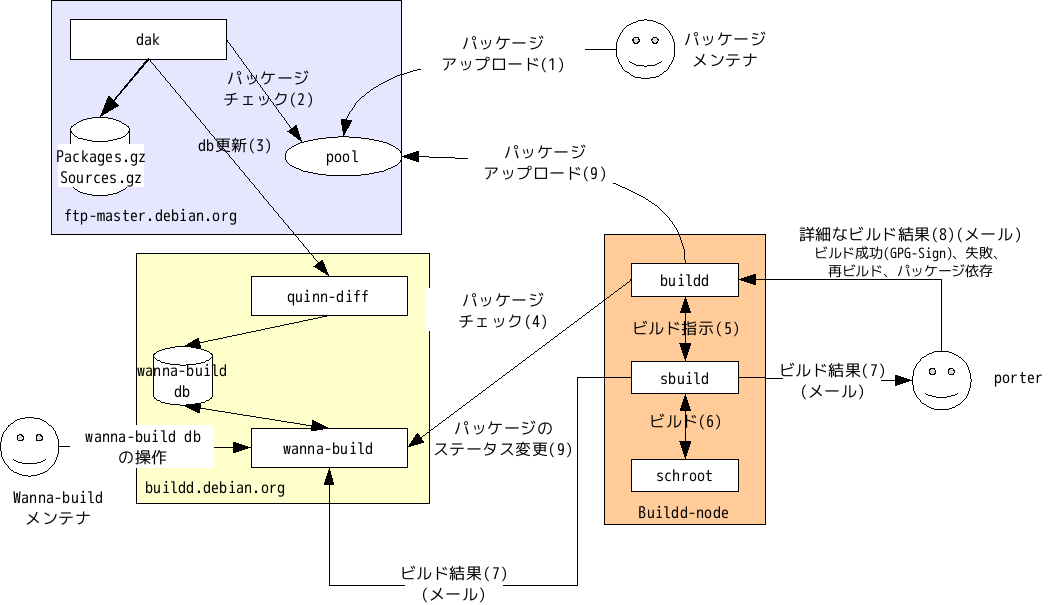
\includegraphics[width=1.1\hsize]{image200911/buildd-image00.png}
\end{center}
\end{frame}

\begin{frame}{パッケージのステータス}
\begin{itemize}
\item BD-Uninstallable
\item Needs-Build 
\item Building 
\item Uploaded
\item Installed
\item Dep-Wait
\item Failed
\item Not-For-Us
\item Failed-Removed
\end{itemize}
\end{frame}

\begin{frame}{ステータスの状態遷移}
\begin{center}
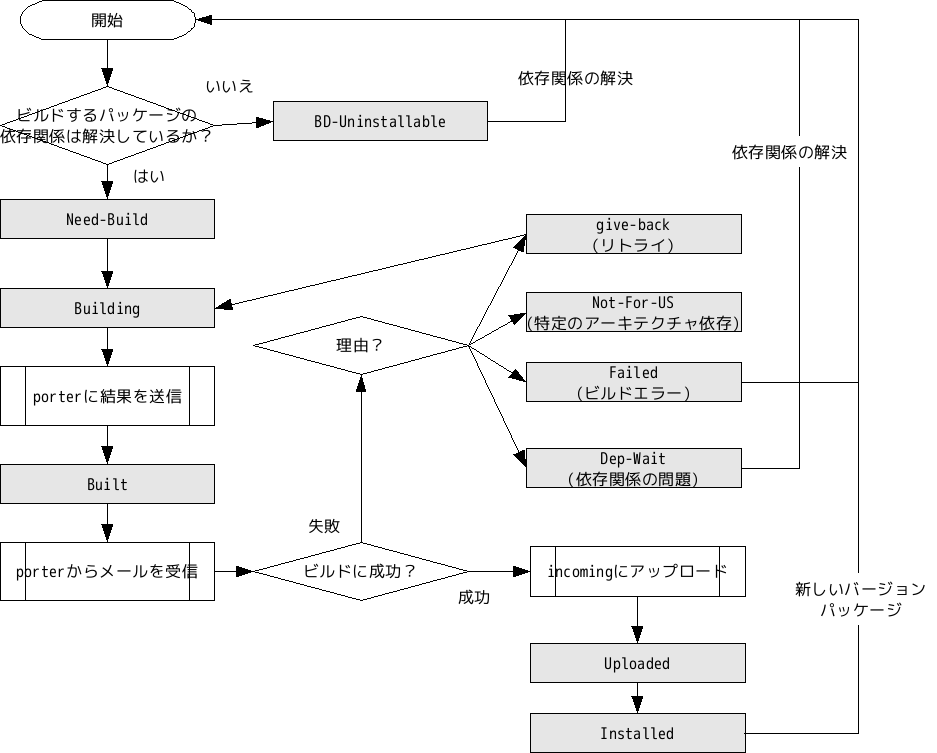
\includegraphics[width=0.9\hsize]{image200911/buildd-status.png}
\end{center}
\end{frame}

\begin{frame}{パッケージビルド優先順位}

パッケージビルドの優先順位が決まっている。
\begin{enumerate}
\item ソースパッケージのプライオリティ
\item ソースパッケージのセクション
\item パッケージ名ASCII 順
\item Need-Build のステータスになった順 
\end{enumerate}

\end{frame}

\begin{frame}{新しいアーキテクチャを追加する}

\begin{itemize}
\item buildd.debian.ort にはすぐには追加することはできない
\item debian-ports.org
\item quinn-diff と wanna-build サービスを提供
\item 現在、hurd-1386, m68k, avr32, sh4 がこのサービスを利用中。
\end{itemize}
\end{frame}



\begin{frame}[containsverbatim]{loop-depends 対応}

\begin{enumerate}
\item loop-depends\\
パッケージがループしてビルド依存している状態。\\

\item 例
\begin{commandline}
- libgtk2-perl -> libpang-perl -> 
        libgtk2-perl -> libpang-perl -> .....
- cups -> avahi -> pygtk -> librsvg -> 
        libgsf -> gnome-vfs  -> gconf -> cups
\end{commandline}

\item 修正方法は決まっていない
\item unreleased ディストリビューションを利用する

\end{enumerate}
\end{frame}


\begin{frame}{loop-depends 対応}
\begin{center}
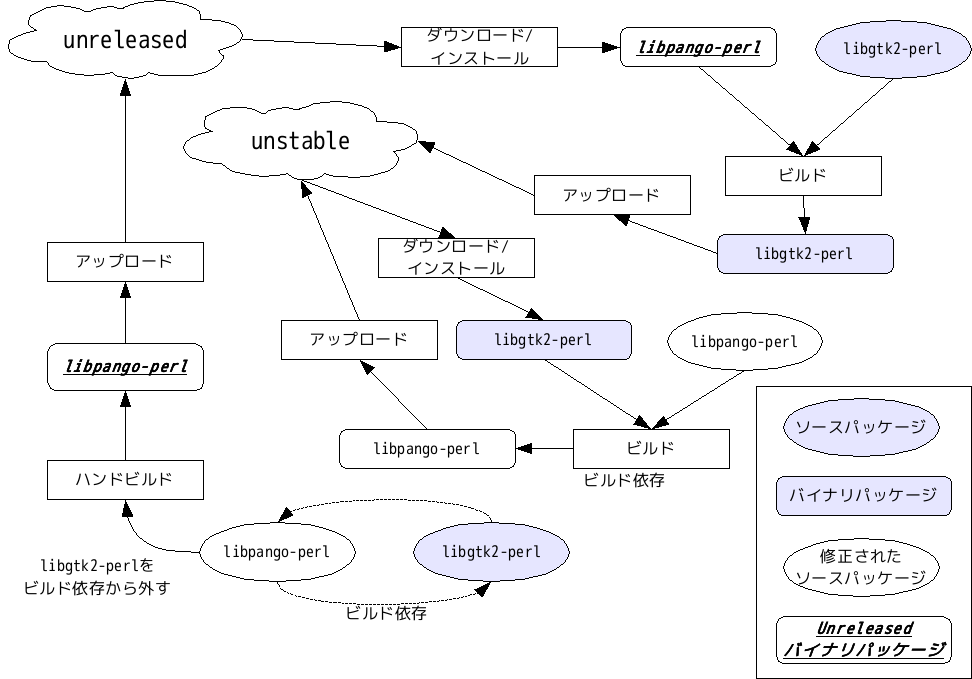
\includegraphics[width=1.1\hsize]{image200911/loop-dep-image.png}
\end{center}
\end{frame}

\begin{frame}{質問}
\begin{center}
\Huge{何か質問はありますか?}
\end{center}
\end{frame}


\end{document}

;;; Local Variables: ***
;;; outline-regexp: "\\([ 	]*\\\\\\(documentstyle\\|documentclass\\|emtext\\|section\\|begin{frame}\\)\\*?[ 	]*[[{]\\|[]+\\)" ***
;;; End: ***
